\documentclass[12pt,a4paper]{report}
%
% This LaTeX template has been created by Luca Grilli
% Based on the following https://en.wikibooks.org/wiki/LaTeX/Title_Creation
%
\usepackage[italian]{babel}
\usepackage[T1]{fontenc}
\usepackage{geometry}
\usepackage{graphicx}
\usepackage{hyperref}
\usepackage[utf8]{inputenc}
\usepackage{subcaption}
\usepackage[nottoc,numbib]{tocbibind}
\usepackage{titlesec}
\usepackage{float}

\titleformat{\chapter}[display]{\Huge\bfseries}{}{0pt}{\thechapter.\ }

\graphicspath{{figures/}}
%
%\addtolength{\topmargin}{-.875in} % reduce the default top margin
%\addtolength{\topmargin}{-2cm} % reduce the default top margin
%



%%%%%%%%%%%%%%%%%%%%%%%%%%%%%%%%%%
%                                %
%     Begin Docuemnt [start]     %
%                                %
%%%%%%%%%%%%%%%%%%%%%%%%%%%%%%%%%%
\begin{document}



%%%%%%%%%%%%%%%%%%%%%%%%%%%%%%
%     Title Page [start]     %
%%%%%%%%%%%%%%%%%%%%%%%%%%%%%%
% Declare new goemetry for the title page only.
\newgeometry{margin=1in}
\begin{titlepage}
	\centering
	\includegraphics[width=0.34\textwidth]{logo-unipg}\par\vspace{1cm}
	\large{Tesina Finale di}\par
	\large{\textbf{Programmazione di Interfacce Grafiche e Dispositivi Mobili}}\par
	\small{Corso di Laurea in Ingegneria Informatica ed Elettronica, Curriculum Informatica} 
	
	\small{A.A. 2021-2022} \par
	\textsc{\small{Dipartimento di Ingegneria}}\par
	%\large{A.A. 2018-2019}\par

	%\vfill
	\vspace{0.5cm}
	docente\par
	Prof.~Luca \textsc{Grilli}

	\vspace{1cm}
	%\textsc{\large{Tesina Finale a.a. 2018-2019}}\par
	\vspace{1cm}
	\textbf{\huge{Fox On The Road}}\par
	\vspace{0.2cm}
	Applicazione Desktop \textsc{JFC/Swing}\par
	%applicazione desktop \textsc{JavaFX}\par
	%app nativa per Android sviluppata con \textsc{AndroidStudio}\par
	\vspace{0.5cm}
	\includegraphics[width=0.40\textwidth]{FoxOnTheRoad_Logo}\par\vspace{1cm}
	\vspace{1cm}

	%\begin{tabular}{ l l l l }
	%\Large{\emph{112233}} & \Large{\emph{Mario}} & \Large{\emph{Rossi}} & \Large{\emph{mario.rossi@studenti.unipg.it}}\\
	%\Large{\emph{114455}} & \Large{\emph{Carlo}} & \Large{\emph{Bianchi}} & \Large{\emph{carlo.bianchi@studenti.unipg.it}}\\
	%\end{tabular}

	\large{studenti}\par
	\vspace{0.2cm}
	\begin{tabular}{ l l l l }
	\large{329118} & \large{\textbf{Francesco}} & \large{\textbf{Mancinelli}} & \large{francesco.mancinelli3@studenti.unipg.it}\\
	\large{329956} & \large{\textbf{Tommaso}} & \large{\textbf{Cosimi}} & \large{tommaso.cosimi@studenti.unipg.it}\\
	\end{tabular}

	%\begin{tabular}{ l l l l }
	%112233 & Mario & Rossi & mario.rossi@studenti.unipg.it\\
	%114455 & Carlo & Bianchi & carlo.bianchi@studenti.unipg.it\\
	%\end{tabular}

	\vfill
	% Bottom of the page
	%{\large \today\par}
	\raggedright
	\small{Data ultimo aggiornamento: \today}
\end{titlepage}
% Ends the declared geometry for the titlepage
\restoregeometry
%%%%%%%%%%%%%%%%%%%%%%%%%%%%
%     Title Page [end]     %
%%%%%%%%%%%%%%%%%%%%%%%%%%%%

%%%%%%%%%%%%%%%%%%%%%%%%%%
%     Indice [start]     %
%%%%%%%%%%%%%%%%%%%%%%%%%%
\tableofcontents
%%%%%%%%%%%%%%%%%%%%%%%%
%     Indice [end]     %
%%%%%%%%%%%%%%%%%%%%%%%%

%%%%%%%%%%%%%%%%%%%%%%%%%%%%%%%%%%%%%%%%%%%%
%     Descrizione del Problema [start]     %
%%%%%%%%%%%%%%%%%%%%%%%%%%%%%%%%%%%%%%%%%%%%
\chapter{Descrizione del Problema}\label{ch:despro}
Questo progetto ha l'obiettivo di ricreare in maniera semplificata e con meccaniche ripensate il famoso gioco per Dispositivi Mobili \emph{Crossy Road}~\cite{wiki:it:CrossyRoad,wiki:en:CrossyRoad}.

Per favorire un'ampia compatibilità su diverse piattaforme hardware e software, l'applicativo implementerà la tecnologia JFC/Swing.

L'applicazione è stata ampiamente testata su piattaforme Windows e *NIX-Like.

Nella realizzazione degli schemi \emph{UML} per la tesina sono stati utilizzati il sito PlantTextUML~\cite{PlantTextUML} ed il software Inkscape~\cite{Inkscape} per la loro successiva conversione da SVG a PDF.

\medskip
Sembra doveroso indicare i principali aspetti del videogioco originale \emph{Crossy Road}~\cite{wiki:it:CrossyRoad,wiki:en:CrossyRoad} nel prossimo paragrafo, così da poter esplicare in maniera più completa la nostra versione semplificata.

%----------------------------------------------
% Sezione: Il Videogioco Mobile Crossy Road [start]
%----------------------------------------------
\section{Il Videogioco Crossy Road}\label{se:gal}
Il videogioco originale presenta una visualizzazione 2.5D, con meccaniche incentrate sull'utilizzo da parte di utenti di dispositivi mobili, e di conseguenza dispone di controlli basati su input touch-screen.

\emph{Crossy Road} presenta un personaggio (inizialmente una gallina) il cui scopo è quello di attraversare la strada, senza ovviamente venire colpita dai veicoli.

Non esiste un'organizzazione a livelli, infatti il giocatore potrà continuare all'infinito finché non viene colpito da un veicolo o cade in una trappola secondaria.

Nel gioco originale, come prima anticipato, i comandi sono \emph{touch-first} e l'utente dovrà fare un tap sullo schermo per muoversi in avanti, o fare uno swipe per muoversi lateralmente.

Il personaggio può muoversi liberamente nella mappa visualizzata, senza vincoli fuorché limiti laterali imposti dalla dimensione dello schermo del dispositivo mobile stesso.

Sarà possibile raccogliere monete durante il percorso, generalmente nascoste in giro per la mappa, che verranno poi utilizzate per sbloccare nuovi personaggi.

Oltre ad esse si potranno trovare invece ostacoli secondari, a partire da alberi e rocce che impediscono il passaggio del personaggio principale.

\begin{figure}[bt]
\begin{subfigure}{.32\textwidth}
  \centering
  \includegraphics[width=.95\linewidth]{snapshot_road}
  %\caption{1a}
  \caption{}
  \label{fig:snap1}
\end{subfigure}%
\begin{subfigure}{.32\textwidth}
  \centering
  \includegraphics[width=.95\linewidth]{snapshot_river}
  %\caption{1a}
  \caption{}
  \label{fig:snap2}
\end{subfigure}%
\begin{subfigure}{.32\textwidth}
  \centering
  \includegraphics[width=.95\linewidth]{snapshot_coin}
  %\caption{1b}
  \caption{}
  \label{fig:snap3}
\end{subfigure}
\caption{Tre screenshot del gioco \emph{Crossy Road}.
	(a) rappresenta lo \emph{stage} principale di gioco: la strada da attraversare.
	(b) rappresenta gli ostacoli secondari come il fiume.
	(c) invece rappresenta gli obiettivi nascosti come le monete da raccogliere.}
\label{fig:fig}
\end{figure}
%----------------------------------------------
% Sezione: Il Videogioco Mobile Crossy Road [end]
%----------------------------------------------


%----------------------------------------
% Sezione: L'applicazione Fox On The Road [start]
%----------------------------------------
\section{L'applicazione Fox On The Road}\label{se:appjgal}
\emph{Fox On The Road} è un applicativo Desktop che, come anticipato, vuole emulare un'esperienza semplificata di \emph{Crossy Road}, ma con un particolare occhio all'utilizzo della tastiera.

L'applicazione presenta un'interfaccia che permette di visualizzare le statistiche di gioco oltre al gioco stesso, il tutto contenuto in un'unica finestra rappresentata tramite un \emph{JFrame}.

L'utente vestirà i panni di una volpe e dovrà affrontare, inizialmente, un \emph{tutorial} che consisterà in un livello guidato allo scopo di impartire i comandi e le meccaniche di gioco che dovrà affrontare.
Dopo di esso, il \emph{gameplay} è concepito come una serie di livelli sempre più impegnativi che metteranno alla prova la bravura dell'utente.

Ovviamente, per raggiungere la fine del livello la volpe non si dovrà far colpire dai veicoli che popolano le strade.
L'obiettivo di ogni livello è arrivare alla fine del percorso senza perdere tutte le vite.

\begin{figure}[H]
	\centering
	\includegraphics[width=1\textwidth, trim=2 2 2 2, clip]{GeneralGUI.png}
	\caption{\emph{Screenshot} dell'Applicazione \emph{Fox On The Road}}
	\label{fig:Screenshot}
\end{figure}

%----------------------------------------
% Sezione: L'applicazione Fox On The Road [end]
%----------------------------------------
%%%%%%%%%%%%%%%%%%%%%%%%%%%%%%%%%%%%%%%%%%
%     Descrizione del Problema [end]     %
%%%%%%%%%%%%%%%%%%%%%%%%%%%%%%%%%%%%%%%%%%



%%%%%%%%%%%%%%%%%%%%%%%%%%%%%%%%%%%%%%%%%%%
%     Specifica dei Requisiti [start]     %
%%%%%%%%%%%%%%%%%%%%%%%%%%%%%%%%%%%%%%%%%%%
%{\let\clearpage\relax \chapter{Specifica dei Requisiti}\label{ch:spereq}}
\chapter{Specifica dei Requisiti}\label{ch:spereq}

L'applicativo \emph{Fox On The Road} dovrà soddisfare la serie di requisiti sotto elencati:

\begin{enumerate}
  \item Possibilità di muovere la volpe utilizzando due diverse combinazioni di tasti (WASD e frecce direzionali).
  \item Presenza di un sottofondo musicale e dei suoni ambientali di gioco.
  \item Presenza di più livelli di gioco con relativa percentuale di completamento.
  \item Presenza di un livello di pratica che mette a disposizione dell'utente un'informativa sulle meccaniche di gioco (\emph{Tutorial}).
  \item Possibilità di estendere il gioco aggiungendo nuovi livelli semplicemente generando un nuovo file di testo che segua la convenzione indicata nel file README.txt.
  \item Possibilità fermare l'avanzamento del timer, di fatto fermando le meccaniche di gioco principali tramite bottone grafico o input da tastiera (Implementazione di uno stato di pausa).
  \item Possibilità di salvare i punteggi più alti.
  \item Presenza di monete posizionate lungo il percorso che permettano di aumentare le vite disponibili.
  \item Presenza di ostacoli statici quali alberi o rocce posizionati lungo il percorso che non permettano all'utente il passaggio.
  \item Presenza di ostacoli mobili generati casualmente quali auto o camion.
  \item Presenza di collisioni del personaggio principale con oggetti statici e dinamici con le relative conseguenze.
  \item Impossibilità di sovrapposizione dei modelli degli ostacoli mobili.
  \item Presenza di texture scelte casualmente per il tappeto erboso, gli ostacoli statici e gli ostacoli dinamici.
  \item Presenza di texture animate per il personaggio principale e per le entità scelte.
  \item Possibilità di visualizzare la mappa di gioco in maniera solidale al movimento della volpe.
  \item Presenza di animazioni fluide per il movimento del personaggio principale e degli ostacoli mobili.
  \item Possibilità di riconoscere l'applicativo aperto nella barra delle applicazioni in esecuzione tramite un'icona personalizzata.
  \item Minimizzazione delle operazioni da terminale, privilegiando l'interfaccia grafica del gioco stesso e l'input da tastiera.
\end{enumerate}
%%%%%%%%%%%%%%%%%%%%%%%%%%%%%%%%%%%%%%%%%
%     Specifica dei Requisiti [end]     %
%%%%%%%%%%%%%%%%%%%%%%%%%%%%%%%%%%%%%%%%%

%%%%%%%%%%%%%%%%%%%%%%%%%%%%
%     Progetto [start]     %
%%%%%%%%%%%%%%%%%%%%%%%%%%%%
\chapter{Progetto}\label{ch:prog}
Viene qua di seguito presentata in maniera esaustiva l'architettura del software e dei suoi singoli blocchi funzionali.

% Architettura del Sistema Software [start]
%-------------------------------------------
\section{Architettura del Sistema Software}\label{ch:arch}
L'architettura software scelta per la realizzazione segue la filosofia Logic-View.

Il package Logic si occupa, come fa sottointendere il termine stesso, dell'implementazione della logica dell'applicazione. Complementarmente, il package View ha la responsabilità di gestire la realizzazione grafica del prodotto.

Per semplicità di implementazione, abbiamo deciso di utilizzare un altro package di supporto chiamato Utilities, che mette a disposizione metodi che fanno riferimento ad operazioni di I/O e metodi non categorizzabili come logici o visualizzativi.

Di seguito mettiamo a disposizione del lettore lo schema UML generale dell'applicativo correlato da una breve descrizione, dopodiché ci concentreremo sugli specifici package.


\begin{figure}[H]
	\centering
	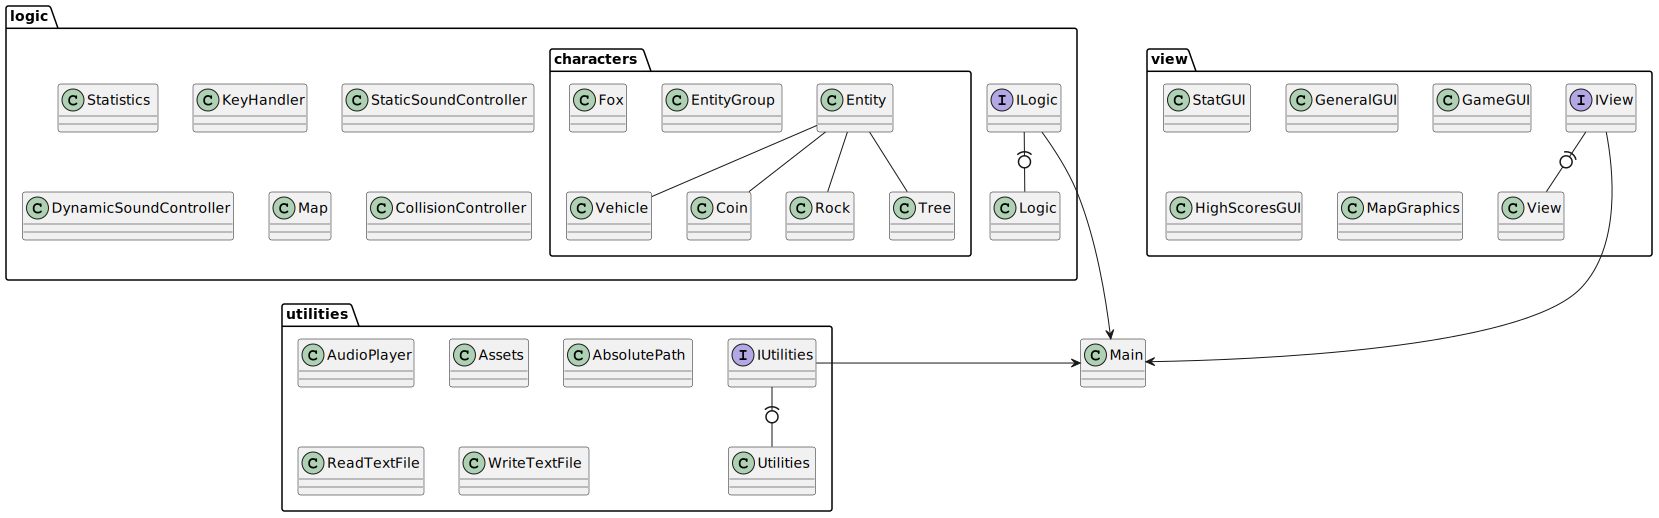
\includegraphics[width=1\textwidth]{Generale.pdf}
	\caption{\emph{Overview} dell'Architettura Software di \emph{Fox On The Road}}
	\label{fig:GeneralUML}
\end{figure}

Come ben si evince dallo schema in Fig.~\ref{fig:GeneralUML} ogni package ha a diposizione un'interfaccia per comunicare con le altre componenti senza avere necessità di condividere le proprie risorse.

Anche le interfacce sono tra loro collegate in quanto all'avvio dell'applicativo viene implementata una funzione di \emph{Injecting} al livello del \emph{Main}, che permetterà ai vari package di accedere a funzioni disponibili nelle altre strutture.

Tutte le classi - ad eccezione di casi particolari - all'interno di un package sono esplicitamente collegate alla classe che materializza l'interfaccia di comunicazione. Questa operazione viene svolta allo scopo di rendere modulare ogni parte del codice, così da renderlo sviluppabile da team indipendenti.

Come risultato di questa operazione, nessuna classe che non sia un'interfaccia (\emph{ILogic}, \emph{IView}, \emph{IUtilities}), è collegata a nulla al di fuori del suo package, eccezion fatta per il collegamento con il \emph{Main} di \emph{Logic}, \emph{View} ed \emph{Utilities}, necessarie all'\emph{Injecting}.

% Architettura del Sistema Software [end]
%-------------------------------------------

% Logic [start]
%-------------------------------------------
\section{Logic}\label{se:arch.model}

Viene riportata immediatamente sotto l'architettura del package \emph{Logic} e del suo sotto-package \emph{Characters}.

\begin{figure}[H]
	\centering
	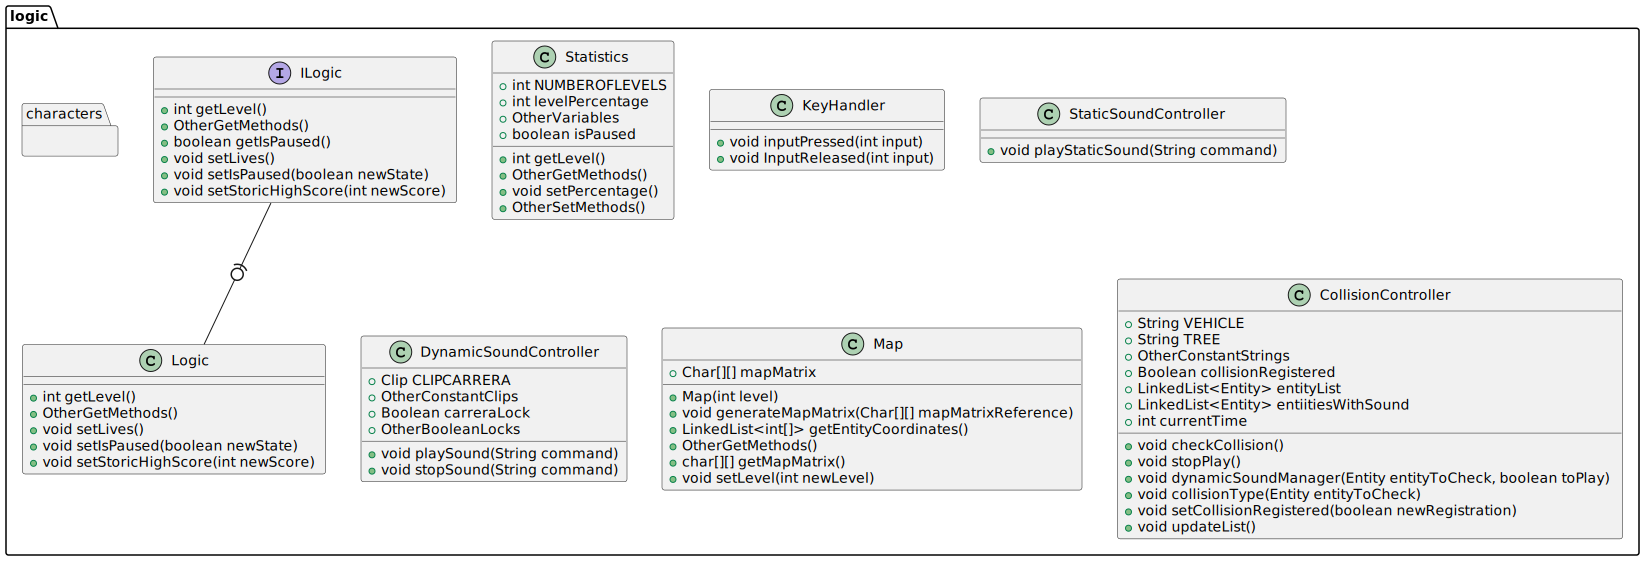
\includegraphics[width=1\textwidth]{LogicWithoutCharacters.pdf}
	\caption{Package \emph{Logic} nella sua interezza}
	\label{fig:Logic}
\end{figure}

\begin{itemize}
	\item Logic 
	\begin{itemize}
		\item Come accennato in precedenza, la classe \emph{Logic} si occupa di collegare le classi interne al suo package con l'interfaccia di comunicazione \emph{ILogic}. A tale collegamento sfuggono \emph{DynamicSoundController} e \emph{StaticSoundController}, che non hanno la necessità di essere richiamate da altri elementi al di fuori della logica.
	\end{itemize}
	\item Statistics
	\begin{itemize}
		\item La classe \emph{Statistics} si occupa di monitorare e modificare le statistiche di gioco e controllare delle meccaniche, come ad esempio il cambio di livello con il metodo \emph{setLevel(int newLevel)}, o la pausa tramite il metodo \emph{setIsPaused(boolean newState)}. 
	\end{itemize}
	\item Map 
	\begin{itemize}
		\item La classe \emph{Map} si occupa della costruzione logica della mappa di gioco, in base ai file di testo che rappresentano gli elementi e le entità, con la loro posizione all'interno di ciascun livello. Oltre ciò restituisce anche il numero di colonne giocabili per ogni livello.
	\end{itemize}
	\item CollisionController
	\begin{itemize}
		\item La classe \emph{CollisionController} si occupa della gestione delle collisioni tra la volpe e le altre entità all'interno dell'applicativo. A seguire, una breve descrizione dei metodi principali:
		\begin{itemize}	
			\item \emph{checkCollision()} verifica che tra l'entità volpe e le altre entità contenute nella Lista \emph{entityList} recuperata dalla classe \emph{Map} non vi siano collisioni. Qualora ne fosse registrata una, il compito di gestirla verrà destinato alla funzione \emph{collisionType()}. Nel caso la volpe invece fosse lontana da entità che generano rumore, il loro suono verrà interrotto da \emph{stopPlay()}.
			\item \emph{collisionType(Entity entityToCheck)} si occupa di controllare di che tipo sia l'entità che è stata colpita o che ha colpito la volpe, prendendo i provvedimenti necessari: ad esempio una collisione con un ostacolo statico come un albero fermerà la volpe, mentre la collisione con un veicolo porterà al reset del livello.
			\item \emph{dynamicSoundManager(Entity entityToCheck, boolean toPlay)} controlla la riproduzione dei suoni delle entità in movimento e degli alberi.
			\item \emph{stopPlay()} interrompe il suono proveniente da entità ora lontane precedentemente in riproduzione.
			\item \emph{updateList()} si occupa di aggiornare la lista delle entità ad ogni cambio livello.
		\end{itemize}
	\end{itemize}
	\item StaticSoundController
	\begin{itemize}
		\item La classe \emph{StaticSoundController} si occupa di riprodurre suoni molto brevi di collisione con rocce e alberi, e raccolta di monete.
	\end{itemize}
	\item DynamicSoundController
	\begin{itemize}
		\item La classe \emph{DynamicSoundController} si occupa di riprodurre il suono ambientale degli alberi ed il rumore di ogni tipo di veicolo. Non è stato deciso di associare ad ogni singolo veicolo una \emph{Clip} per motivi prestazionali e di sound design, perciò ci sarà una \emph{Clip} per ogni tipologia di veicolo.
	\end{itemize}
	\item KeyHandler
	\begin{itemize}
		\item La classe \emph{KeyHandler} si occupa di gestire gli input da tastiera per poi restituirli alla classe \emph{Fox} - contenuta nel sotto-package \emph{Characters} - che li utilizzerà per muovere la volpe.
	\end{itemize}
\end{itemize}

Viene riportata immediatamente sotto l'architettura del sotto-package \emph{Characters}, contenuto nel package \emph{Logic}.
\begin{figure}[H]
	\centering
	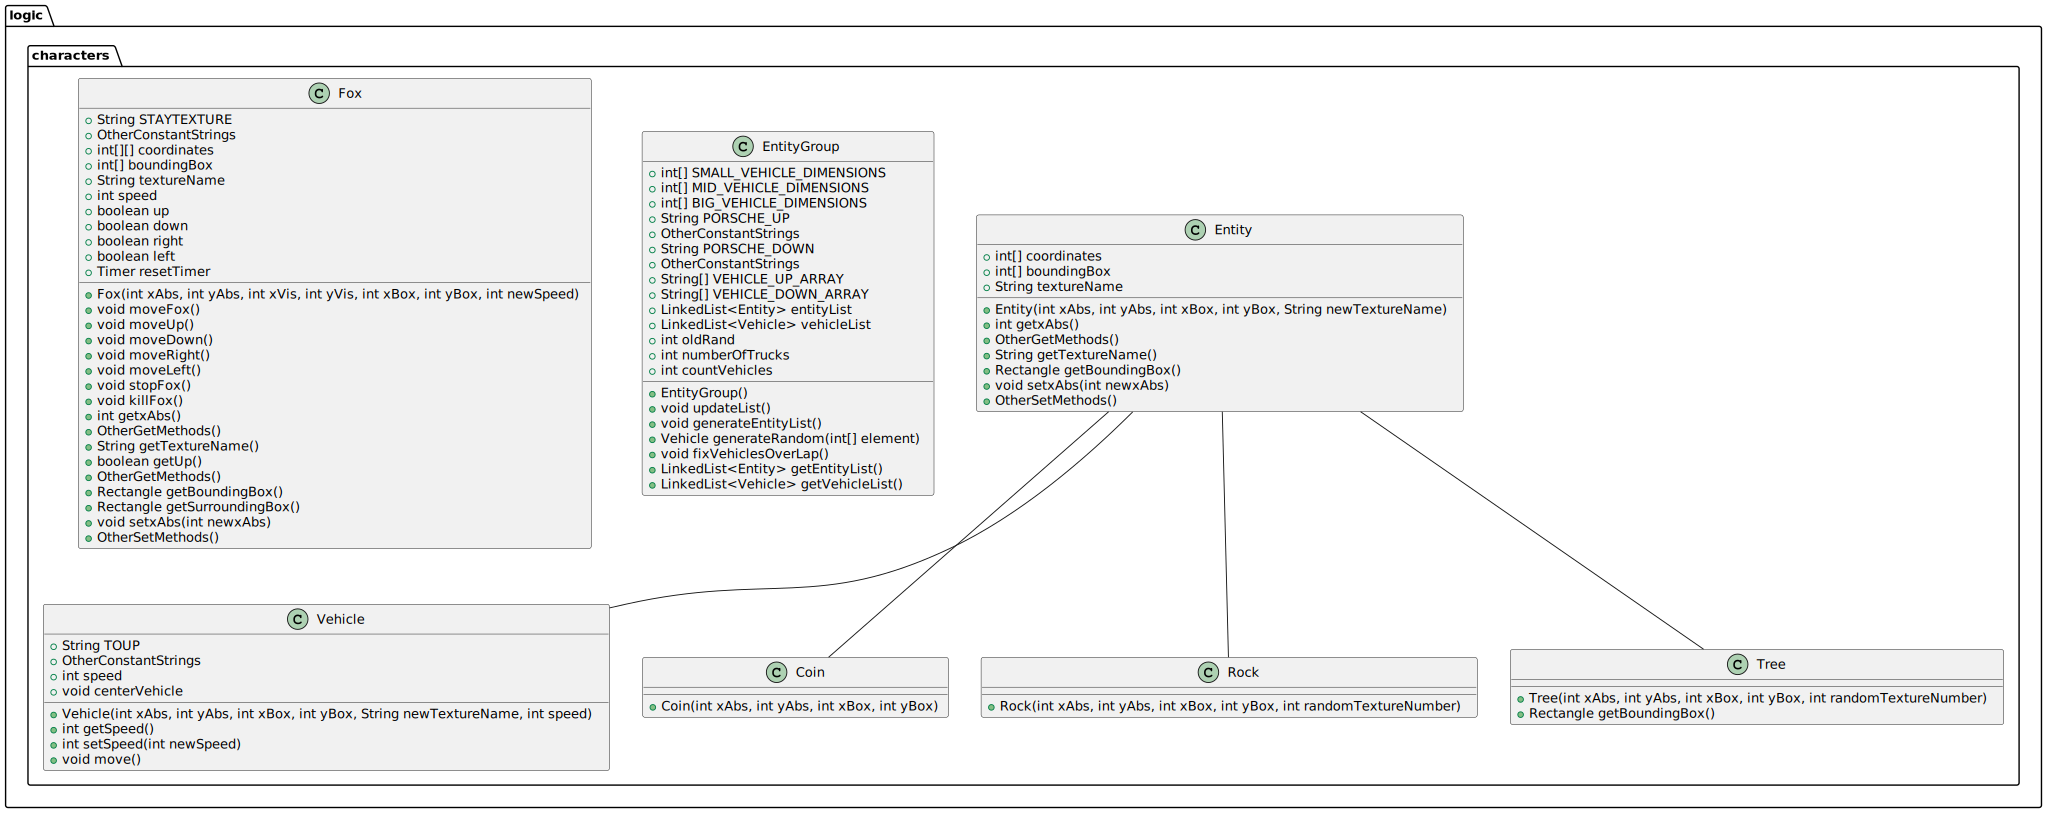
\includegraphics[width=1\textwidth]{Characters.pdf}
	\caption{Sotto-package \emph{Characters} di \emph{Logic}}
	\label{fig:Characters}
\end{figure}

\begin{itemize}
	\item Fox
	\begin{itemize}
		\item La classe \emph{Fox} rappresenta il concetto logico di volpe all'interno dell'applicativo. Si occupa del movimento e degli stati della volpe. Il movimento è affidato ai metodi \emph{moveFox()}, \emph{moveUp()}, \emph{moveDown()}, \emph{moveRight()} e \emph{moveLeft()}, invece gli stati della volpe sono affidati ai metodi \emph{killFox()}, \emph{stopFox()} e ai metodi di movimento che si appoggiano al metodo \emph{setTextureName()}.
	\end{itemize}
	\item Entity
	\begin{itemize}
		\item La classe \emph{Entity} è una generalizzazione delle varie classi \emph{Coin}, \emph{Rock},\emph{Tree} e \emph{Vehicle}.
	\end{itemize}
	\item Coin
	\begin{itemize}
		\item La classe \emph{Coin} rappresenta il concetto logico di moneta all'interno dell'applicativo.
	\end{itemize}
	\item Rock
	\begin{itemize}
		\item La classe \emph{Rock} rappresenta il concetto logico di roccia all'interno dell'applicativo.
	\end{itemize}
	\item Tree
	\begin{itemize}
		\item La classe \emph{Tree} rappresenta il concetto logico di albero all'interno dell'applicativo.
	\end{itemize}
	\item Vehicle
	\begin{itemize}
		\item La classe \emph{Vehicle} rappresenta il concetto logico di veicolo all'interno dell'applicativo. Essendo però elementi dinamici, hanno a disposizione un attributo che rappresenta la loro velocià ed un metodo \emph{move()} che permetta il movimento.
	\end{itemize}
	\item EntityGroup
	\begin{itemize}
		\item La classe \emph{EntityGroup} si occupa della generazione delle entità con \emph{texture} e \emph{hitbox} associate casuali, delle loro liste e della gestione delle collisioni tra entità dinamiche (veicoli). Di seguito vengono riportate le descrizioni di alcuni dei metodi principali:
		\begin{itemize}
			\item Il costruttore \emph{EntityGroup()} va a generarsi immediatamente la lista di Entità tramite il metodo \emph{generateEntityList()}.
			\item Il metodo \emph{generateEntityList()} genera una lista collegata contenente tutte le entità - statiche e dinamiche - presenti nel livello. Provvede anche al riempimento di un'altra lista adibita solo ai veicoli.
			\item Il metodo \emph{fixVehiclesOverlap()} ha il compito di controllare che le entità dinamiche non si sovrappongano ed eventualmente spostarne indietro una delle due.
			\item Il metodo \emph{generateRandom(int[] element)} ha il compito di generare casualmente dei nomi di \emph{texture} che si riferiranno - sul package \emph{View} - a delle \emph{texture} specifiche.
			\item I metodi \emph{flushList()} e \emph{updateList()} hanno rispettivamente il compito di svuotare la lista ad ogni cambio di livello e di aggiornarla.
		\end{itemize}
	\end{itemize}
\end{itemize}



% Logic [end]
%-------------------------------------------

% View [start]
%-------------------------------------------
\section{View}\label{se:arch.view}

Viene riportata immediatamente sotto l'architettura del package \emph{View}.

\begin{figure}[H]
	\centering
	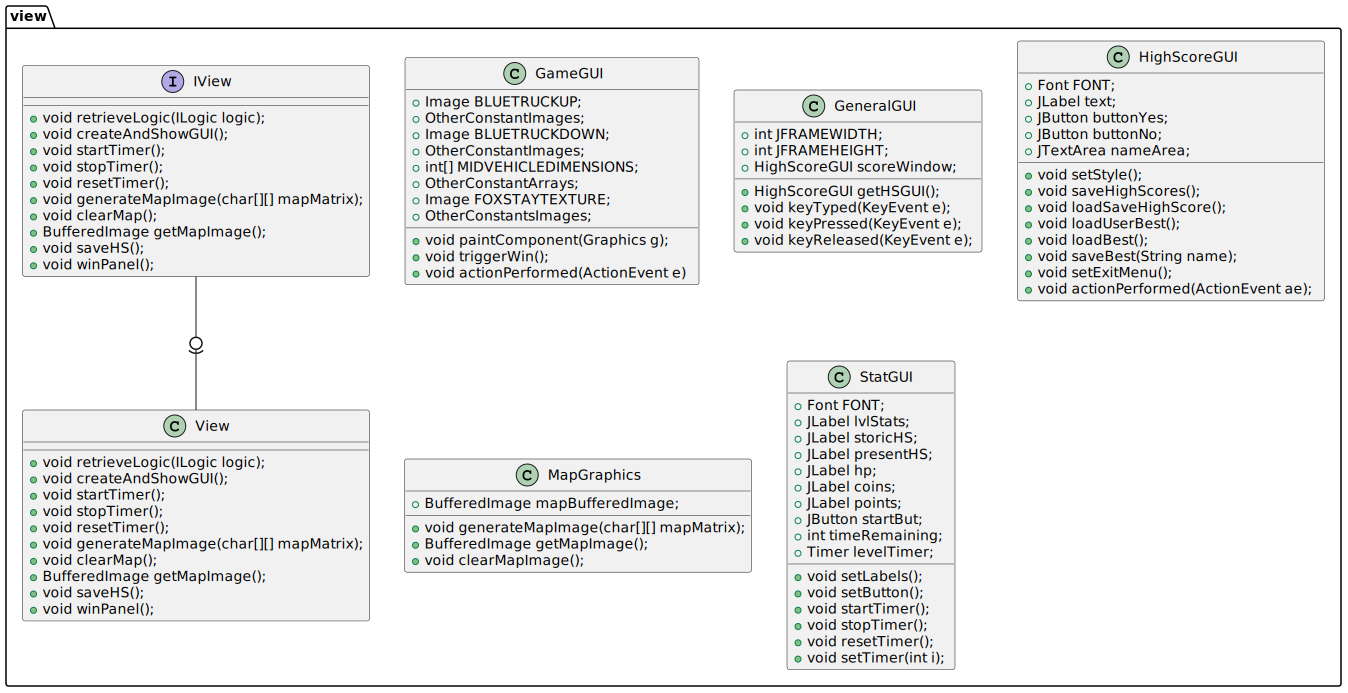
\includegraphics[width=1\textwidth]{View.pdf}
	\caption{Package \emph{View} nella sua interezza}
	\label{fig:View}
\end{figure}

\begin{itemize}
	\item GeneralGUI
	\begin{itemize}
		\item La classe \emph{GeneralGUI} si occupa di contenere i sottopannelli \emph{GameGUI}, \emph{StatGUI} e \emph{HighScoreGUI} all'interno di un'unica finestra. Oltre ciò si occupa di estendere il \emph{KeyListener} per catturare gli input dell'utente da trasferire successivamente alla classe \emph{KeyHandler} nel package \emph{Logic}.
		\begin{figure}[H]
			\centering
			\includegraphics[width=1\textwidth, trim=2 2 2 2, clip]{GeneralGUI.png}
			\caption{\emph{Screenshot} di \emph{Fox On The Road}, viene mostrata la GeneralGUI}
			\label{fig:GeneralGUI}
		\end{figure}
	\end{itemize}
	\item GameGUI
	\begin{itemize}
		\item La classe \emph{GameGUI} si occupa di visualizzare gli elementi grafici del gioco tramite il metodo \emph{paintComponent()}, che li visualizza nel suo \emph{JPanel}. Grazie ai metodi della classe astratta \emph{ActionListener}, è stato impostato un timer di 16ms (62,5 Frame per Secondo) che richiama nuovamente il \emph{paintComponent()}, permettendo il refresh della grafica. Alcuni elementi non sono sempre visualizzati, tra di loro spiccano l'\emph{overlay} del tutorial e l'immagine di vittoria.
		\begin{figure}[H]
			\centering
			\includegraphics[width=1\textwidth, trim=2 2 2 2, clip]{GameGUI.png}
			\caption{Dimostrazione del funzionamento della classe \emph{GameGUI}}
			\label{fig:GameGUI}
		\end{figure}
	\end{itemize}
	\item StatGUI
	\begin{itemize}
		\item La classe \emph{StatGUI} si occupa di visualizzare le statistiche della partita all'interno della finestra del gioco, accompagnandole ad un \emph{JButton} che ha come \emph{Label} un timer di livello che permetta di far andare il gioco in uno stato di pausa. Tra le statistiche visualizzate spiccano i punteggi migliori, le vite rimanenti e le monete raccolte.
		\begin{figure}[H]
			\centering
			\includegraphics[width=1\textwidth, trim=2 2 2 2, clip]{StatGUI.png}
			\caption{Dimostrazione del funzionamento della classe \emph{StatGUI}}
			\label{fig:StatGUI}
		\end{figure}
	\end{itemize}
	\item HighScoreGUI
	\begin{itemize}
		\item La classe \emph{HighScoreGUI} implementa un \emph{JPanel} che permette all'utente di salvare e/o caricare i migliori punteggi. Permette anche l'inserimento di nomi personalizzati, in modo da stilare una classifica consultabile tramite l'apposito file CSV nella cartella \emph{Assets/Misc}.
		\begin{figure}[H]
			\begin{subfigure}{0.5\textwidth}
				\centering
				\includegraphics[width=1\textwidth, trim=2 2 2 2, clip]{HSGUI_Load.png}
				\caption{Richiesta di caricamento del miglior punteggio personale}
				\label{fig:HSGUILoad}
			\end{subfigure}
			\begin{subfigure}{0.5\textwidth}
				\centering
				\includegraphics[width=1\textwidth, trim=2 2 2 2, clip]{HSGUI_Name.png}
				\caption{Richiesta del nome a seguito di una risposta affermativa}
				\label{fig:HSGUILoad}
			\end{subfigure}
			\caption{Dimostrazione del funzionamento della classe \emph{HighScoreGUI}}
		\end{figure}
	\end{itemize}
	\item MapGraphics
	\begin{itemize}
		\item La classe \emph{MapGraphics} riceve in input la mappa logica generata dalla classe \emph{Map} nel package \emph{Logic} e produce in output le grafiche della mappa, assegnando ad ogni elemento della matrice la \emph{texture} appropriata scelta in maniera casuale. Oltre alla mappa pura e semplice, si occupa di piazzare nella locazione desiderata e di assegnare le \emph{texture} corrispondenti alle entità statiche contenute nel file della mappa.
	\end{itemize}
\end{itemize}

% View [end]
%-------------------------------------------

% Utilities [start]
%-------------------------------------------
\section{Utilities}\label{se:arch.model}

Viene riportata immediatamente sotto l'architettura del package \emph{Utilities}.

\begin{figure}[H]
	\centering
	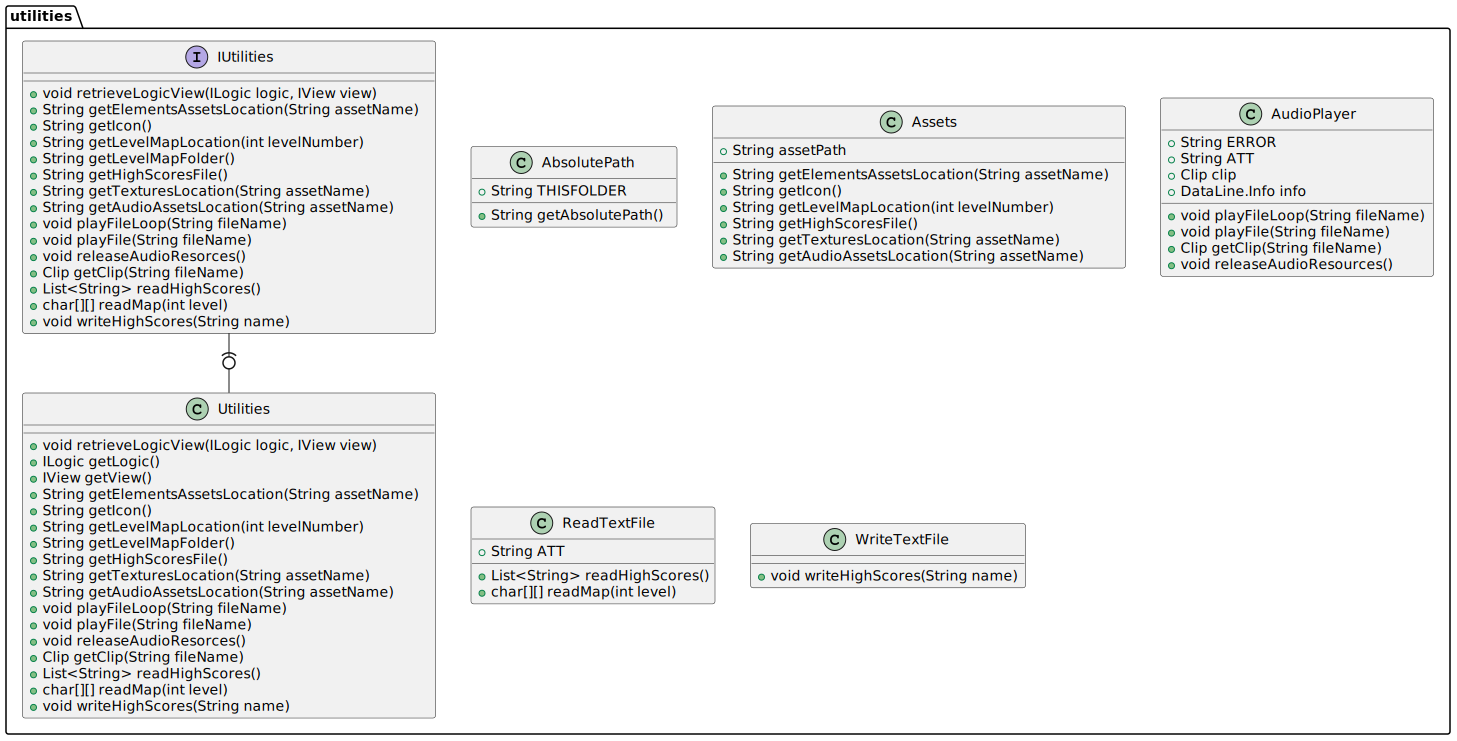
\includegraphics[width=1\textwidth]{Utilities.pdf}
	\caption{Package \emph{Utilities} nella sua interezza}
	\label{fig:Utilities}
\end{figure}

\begin{itemize}
	\item AbsolutePath
	\begin{itemize}
		\item La classe \emph{AbsolutePath} si occupa esportare come stringa la posizione assoluta nel \emph{File System}.
	\end{itemize}
	\item Assets
	\begin{itemize}
		\item La classe \emph{Assets} si occupa di restituire le locazioni assolute delle risorse richieste facendo affidamento sulla posizione indicata da \emph{AbsolutePath}.
	\end{itemize}
	\item ReadTextFile
	\begin{itemize}
		\item La classe \emph{ReadTextFile} permette di leggere i \emph{file CSV} e \emph{TXT}, quindi si occupa di leggere il file con i punteggi migliori ed i file delle mappe.
	\end{itemize}
	\item WriteTextFile
	\begin{itemize}
		\item La classe \emph{WriteTextFile} permette di scrivere su \emph{file CSV}, quindi si occupa di scrivere sul file con i punteggi migliori.
	\end{itemize}
	\item AudioPlayer
	\begin{itemize}
		\item La classe \emph{AudioPlayer} permette di riprodurre \emph{file} audio in formato \emph{WAV} una sola volta o in \emph{loop}, o di restituire le \emph{Clip} per la loro riproduzione al di fuori di \emph{Utilities}. Esempio eclatante sono quelle riprodotte all'interno di \emph{DynamicSoundController} e \emph{StaticSoundController}.
	\end{itemize}
\end{itemize}


% Utilities [end]
%-------------------------------------------

% Problemi Riscontrati [start]
%-------------------------------------------
\section{Problemi Riscontrati}\label{ch:proris}
% Problemi Riscontrati [end]
L'implementazione della logica di \emph{Fox On The Road} non ha sollevato problemi ingenti, tuttavia non si può dire che sia stata un'avventura senza imprevisti.

Dato che non avevamo un grande bagaglio culturale dal punto di vista della programmazione al di fuori dell'ambito universitario, i problemi più impegnativi si sono presentati nel primo momento di stesura e progettazione del codice del software:
in particolare nel momento in cui dovevamo visualizzare le entità sopra al manto erboso che costituisce la base della visualizzazione grafica della \emph{GameGUI}, ad esempio.

Si riportano di seguito alcuni dei più impegnativi (per noi) problemi riscontrati durante la stesura del codice:
\begin{itemize}
\item Gestione dell'accesso concorrenziale delle liste, che contengono le entità che devono essere visualizzate nella posizione allocata nella mappa di gioco, risolto copiando la lista e scorrendo la copia;
\item Gestione delle risorse sonore per le entità, risolto aggiustando l'implementazione delle \emph{Clip} da riprodurre;
\item Gestione delle collisioni delle entità con il personaggio principale, in particolare riferiti alla collissione tra la texture della volpe e quelle delle entità statiche, che venivano inizialmente sovrapposte. Questo problema è stato risolto nella classe \emph{CollisionController} spostando indietro la volpe ogni qual volta ci fosse un'interazione tra i due;
\item Gestione della sovrapposizione dei veicoli, che essendo generati randomicamente e tutti nella stessa posizione iniziale, potevano sovrapporsi in maniera non consona, è stato risolto nella funzione \emph{FixVehiclesOverlap()} nella classe \emph{EntityGroup};
\item Gestione di JPanel atti all'interazione con l'utente ma che non sono fissi, in quanto presenti solamente nei casi in cui l'utente voglia caricare il suo miglior punteggio o debba uscire dall'applicazione salvando i progressi fatti, implementato nella classe \emph{HighScoresGUI};
\item Generazione della mappa tramite \emph{tile} di \emph{BufferedImage} che vanno uniti in un'unica \emph{BufferedImage}, problemi risolti nella classe \emph{MapGraphics} dell'applicativo;
\item Gestione del cambio dei livelli e lo svuotamento delle liste contenenti le entità del livello precedente, nonché il cambio di mappa, criticità risolte grazie al metodo \emph{setLevel()} presente nella classe \emph{Statistics};
\item Fluidità del movimento della volpe, che inizialmente era stata implementata tramite il semplice \emph{KeyListener}, senza supporto dal \emph{KeyHandler} ed anche grazie alla presenza di GIF che accompagnino il rispettivo movimento, creando una scena più dinamica.
\end{itemize}

% Problemi Riscontrati [stop]
%-------------------------------------------
%%%%%%%%%%%%%%%%%%%%%%%%%%
%     Progetto [end]     %
%%%%%%%%%%%%%%%%%%%%%%%%%%



%%%%%%%%%%%%%%%%%%%%%%%%%%%%%%%%%%%%%%%%%%%%%%%%%
%     Conclusioni e sviluppi futuri [start]     %
%%%%%%%%%%%%%%%%%%%%%%%%%%%%%%%%%%%%%%%%%%%%%%%%%
\chapter{Conclusioni e sviluppi futuri}\label{ch:conc-svil-fut}

\section{Possibilità di estensione e personalizzazione}
L'applicazione \emph{Fox On The Road} è stata concepita come espandibile sin dall'inizio, con possibilità di aggiungere nuovi livelli semplicemente generando un file di testo da dieci righe con gli elementi indicati nella nostra guida "README.txt".

Viene data all'utente dunque la possibilità di personalizzare, estendere o addirittura eliminare i livelli già presenti e continuare il gameplay creandone altri, senza dover inserire una singola riga di codice nei file sorgente, per questo l'applicazione verrà distribuita esclusivamente nel formato \emph{.jar}.

Oltre al rinnovamento nella struttura dei livelli, è disponibile la personalizzazione del lato estetico e/o sonoro, quindi delle \emph{Texture} di gioco, e delle \emph{SoundTrack}.

Ad esempio, sostituendo i file originali delle \emph{Texture} con altri personalizzati che seguano i requisiti specificati nel file \emph{README.txt} c'è la possibilità di avere un'esperienza di gioco medesima con i personaggi che più vi aggradano.


\section{Sviluppi Futuri}
Proprio per merito dell'espandibilità di cui si è parlato poc'anzi, l'utente finale - o chi per lui - ha la possibilità di espandere come vuole il gioco, rinnovandone il \emph{gameplay}, la veste grafica e/o sonora, il tutto mantenendo le meccaniche di gioco previste in fase di progettazione, e senza toccare codice sorgente.


%%%%%%%%%%%%%%%%%%%%%%%%%%%%%%%%%%%%%%%%%%%%%%%
%     Conclusioni e sviluppi futuri [end]     %
%%%%%%%%%%%%%%%%%%%%%%%%%%%%%%%%%%%%%%%%%%%%%%%


%%%%%%%%%%%%%%%%%%%%%%%%%%%%%%%%%%%%%%%%%%%%%
%     Bibliografia e Sitografia [start]     %
%                 NO BibTeX                 %
%%%%%%%%%%%%%%%%%%%%%%%%%%%%%%%%%%%%%%%%%%%%%
%\chapter{Bibliografia e Sitografia}\label{ch:bibsit}
%
%\begin{thebibliography}{9}
%\bibitem{lamport94}
%  Leslie Lamport,
%  \textit{\LaTeX: a document preparation system},
%  Addison Wesley, Massachusetts,
%  2nd edition,
%  1994.
%\end{thebibliography}
%
%%%%%%%%%%%%%%%%%%%%%%%%%%%%%%%%%%%%%%%%%%%
%     Bibliografia e Sitografia [end]     %
%                 NO BibTeX               %
%%%%%%%%%%%%%%%%%%%%%%%%%%%%%%%%%%%%%%%%%%%



%%%%%%%%%%%%%%%%%%%%%%%%%%%%%%%%%%%%%%%%%%%%%
%     Bibliografia e Sitografia [start]     %
%                with BibTeX                %
%%%%%%%%%%%%%%%%%%%%%%%%%%%%%%%%%%%%%%%%%%%%%
\bibliographystyle{plain}
\bibliography{bibliografia}
% inserire i riferimenti bibliografici nel file 'bibliografia.bib'
%%%%%%%%%%%%%%%%%%%%%%%%%%%%%%%%%%%%%%%%%%%
%     Bibliografia e Sitografia [end]     %
%                with BibTeX              %
%%%%%%%%%%%%%%%%%%%%%%%%%%%%%%%%%%%%%%%%%%%



\end{document}
%%%%%%%%%%%%%%%%%%%%%%%%%%%%%%%%
%                              %
%     Begin Document [end]     %
%                              %
%%%%%%%%%%%%%%%%%%%%%%%%%%%%%%%%